%====================================================
% 第4章：実験・評価
%====================================================
\section{シミュレーション}

\subsection{疑似dq変換}
三相NPP型3レベルインバータを用いた系統連系システムにMSDB制御を適用して，
疑似dq変換のシミュレーションを行う．
Table~.\ref{tab:grid}にシミュレーション条件を示す．
三相系統電圧$V_s$のU相に対して10MHzベースの疑似dq変換を行い，定常状態時における周波数変動率を評価する．
\eqref{eq:12}式に周波数変動率の定義式を示す．周波数変動率とは，定常状態の系統周波数50Hzに対し、
検出された周波数成分の最大値$f_{max}$[Hz]と最小値$f_{min}$[Hz]の差を100分率で表したものである\cite{ref07}．

\begin{equation}
周波数変動率 = \frac{f_{max}-f_{min}}{50}×100 [\%]\label{eq:12} 
\end{equation}


\begin{table}[htbp]
  \centering
  \captionsetup{labelsep=space, name=Table.,skip = 0pt}
  \caption{Simulation conditions}
  \label{tab:grid}
  \begin{tabular}{c|c|c}
    \hline \hline
    Condition & Parameter & Value \\ \hline
    Sampling frequency        & $f_s$   & 1.0~[MHz] \\\hline
    Carrier frequency         & $f_c$   & 3.6~[kHz] \\\hline
    Nominal capacity          & $P$     & 2.0~[MVA] \\\hline
    Grid voltage (RMS)        & $V_s$   & 510~[V] \\\hline
    Operating frequency       & $f$     & 50~[Hz] \\\hline
    DC power supply           & $E_{DC}$& 1100~[V] \\\hline
    Filter inductor           & $L_1$   & 20~[$\mu$H] \\\hline
    Filter capacitor          & $C$     & 1800~[$\mu$F] \\\hline
    Interconnection inductor  & $L_t$   & 20~[$\mu$H] \\\hline
    PLL P Gain                & $KP$    & 0.02  \\\hline
    PLL I Gain                & $KI$    & 0.001 \\\hline
  \end{tabular}
\end{table}


Fig.\ref{fig:grid_wave.png}に
系統電圧$V_s$，コンデンサ電圧$V_C$，インダクタ電流$I_{L1}$，出力電流$I_o$，
$VCO$の出力波形を示す．
Fig.\ref{fig:quasi_dq_sim}に系統電圧$V_s$の$U$相に対して10MHzベースの疑似dq変換によるPLL制御
のシミュレーション結果を示す．
$V_d$[V]は振幅，$V_q$[rad]は位相差，$f1_u$は周波数である．
Table~.\ref{tab:Detection}に周波数変動率を示す．
Table~.\ref{tab:Detection}の結果より，
10MHzベースのPLL制御は1MHzベースのPLL制御に比べ周波数変動率が0.302[\%]抑制できていることがわかる．


\begin{figure}[htbp]
    \centering
     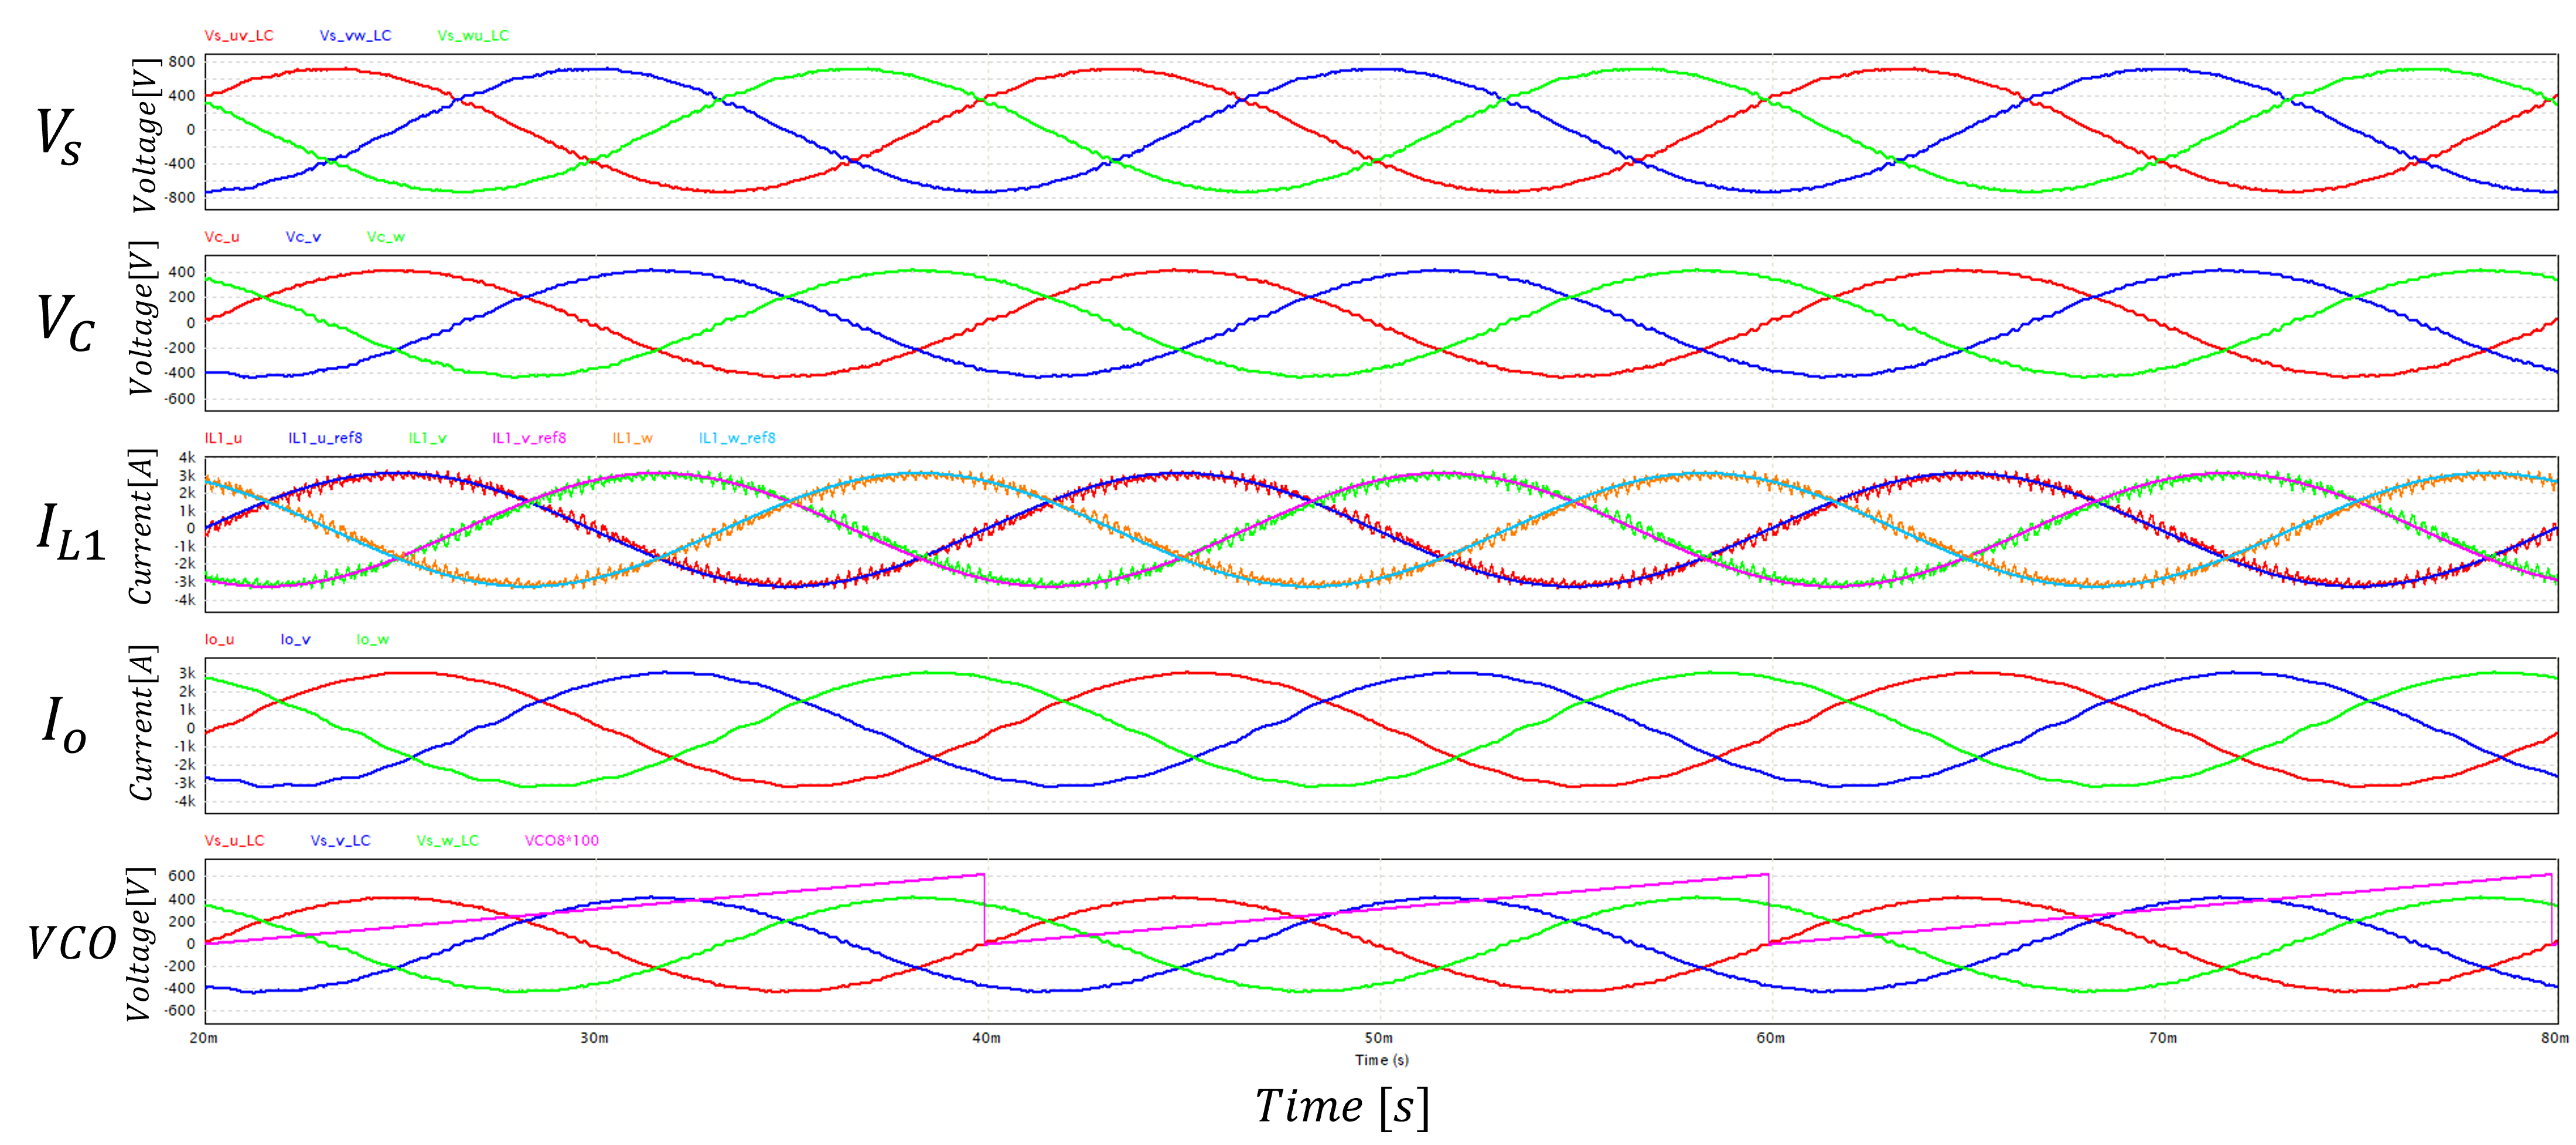
\includegraphics[width=0.5\textwidth]{figures/grid_wave.png}
    \caption{Simulation results of MSDB control}
    \label{fig:grid_wave.png}
\end{figure}


\begin{figure}[htbp]
    \centering
     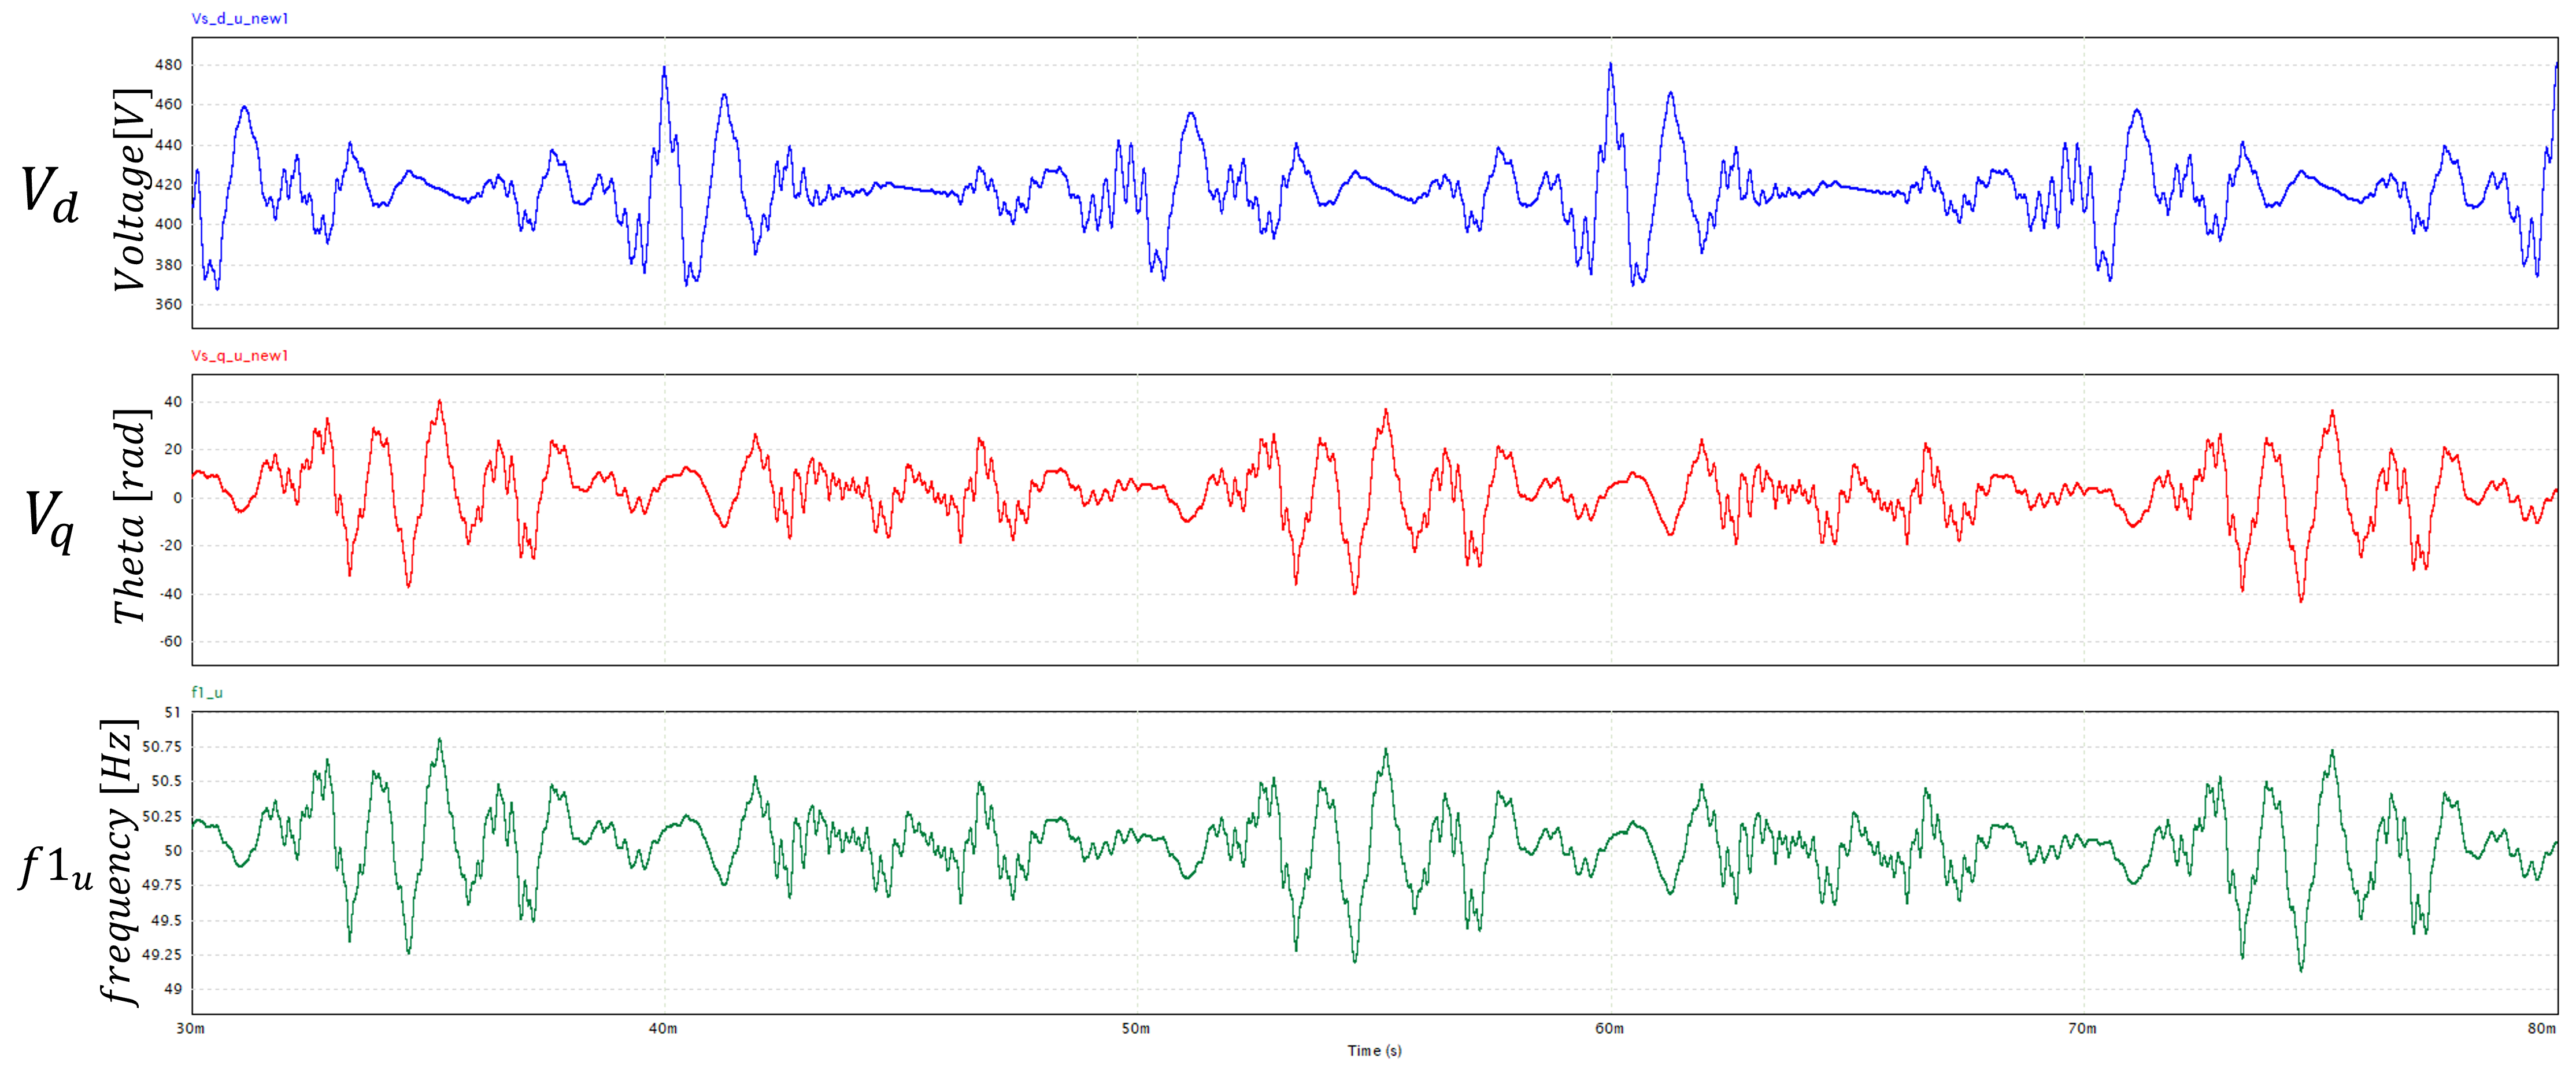
\includegraphics[width=0.5\textwidth]{figures/quasi_dq_sim.png}
    \caption{Simulation results of 10MHz quasi d-q transformation}
    \label{fig:quasi_dq_sim}
\end{figure}


\begin{table}[htbp]
  \centering
    \captionsetup{labelsep=space, name=Table.,skip = 0pt}
  \caption{frequency variation rate}
  \label{tab:Detection}
  \begin{tabular}{c|c}
    \hline \hline
                & frequency variation rate [\%] \\ \hline
    10MHz PLL  & 3.192[\%] \\ \hline
    1MHz PLL & 3.494[\%]  \\ \hline
  \end{tabular}
\end{table}

\subsection{複素係数フィルタ}

単相入力信号$u(t)$を振幅$A$=1[V] ,周波数$f_o$=50[Hz]，初期位相$\theta_o$=0[rad]として
複素係数バンドパスフィルタのシミュレーションを行う.
Table~.\ref{tab:simulation_conditions}にパラメータを示す．



\begin{table}[htbp]
  \centering
    \captionsetup{labelsep=space, name=Table.,skip = 0pt}
  \caption{Simulation conditions}
  \label{tab:simulation_conditions}
  \begin{tabular}{c|c|c}
    \hline \hline
    Condition & Parameter & Value \\ \hline
    Sampling frequency & $f_s$ & 10~[kHz] \\ \hline
    Central frequency & $f_0$ & 50~[Hz] \\ \hline
    Central angular frequency & $\Omega_d$ & 0.314 \\ \hline
    Pass-band bandwidth &$r$& 0.999\\ \hline 
    Amplitude (MAX) & $A$ & 1~[V] \\ \hline
  \end{tabular}
\end{table}

Fig.\ref{fig:without}に高調波を重畳しない場合，Fig.\ref{fig:with}に入力信号に対して，5次高調波20$\%$，11次高調波30$\%$
を重畳した場合，Fig.\ref{fig:f_step}に周波数を50Hzから55Hzにステップ変化させた場合のシミュレーション結果を示す．$u(t)$は入力信号，$y(t)$は瞬時複素ベクトル$V_{re}$，$V_{im}$である．
Fig.\ref{fig:without}，Fig.\ref{fig:with}より，複素係数フィルタを用いることによって，
高調波の重畳に関わらず瞬時複素ベクトル$V_{re} ，V_{im}$を算出できていることが確認できる．
この結果から，複素係数フィルタを用いることで，低次高調波の耐性を有するPLL制御を構成できると考えられる．
Fig.\ref{fig:f_step}より，周波数ステップ変化した直後に出力$y(t)$の振幅が減衰しているが，
フィルタの通過帯域幅を決定するパラメータ$r$を0.999と大きく設定しているため，
瞬時に複素ベクトル$V_{re} ，V_{im}$を算出できていないことが確認できる．
通過帯域幅$r$を小さくすることで応答性は良くなるが，
周波数ステップ成分を十分に除去できない．
ゲイン特性と追従特性の関係を考慮して通過帯域幅$r$を設計する必要がある．



\begin{figure}[htbp]
    \centering
     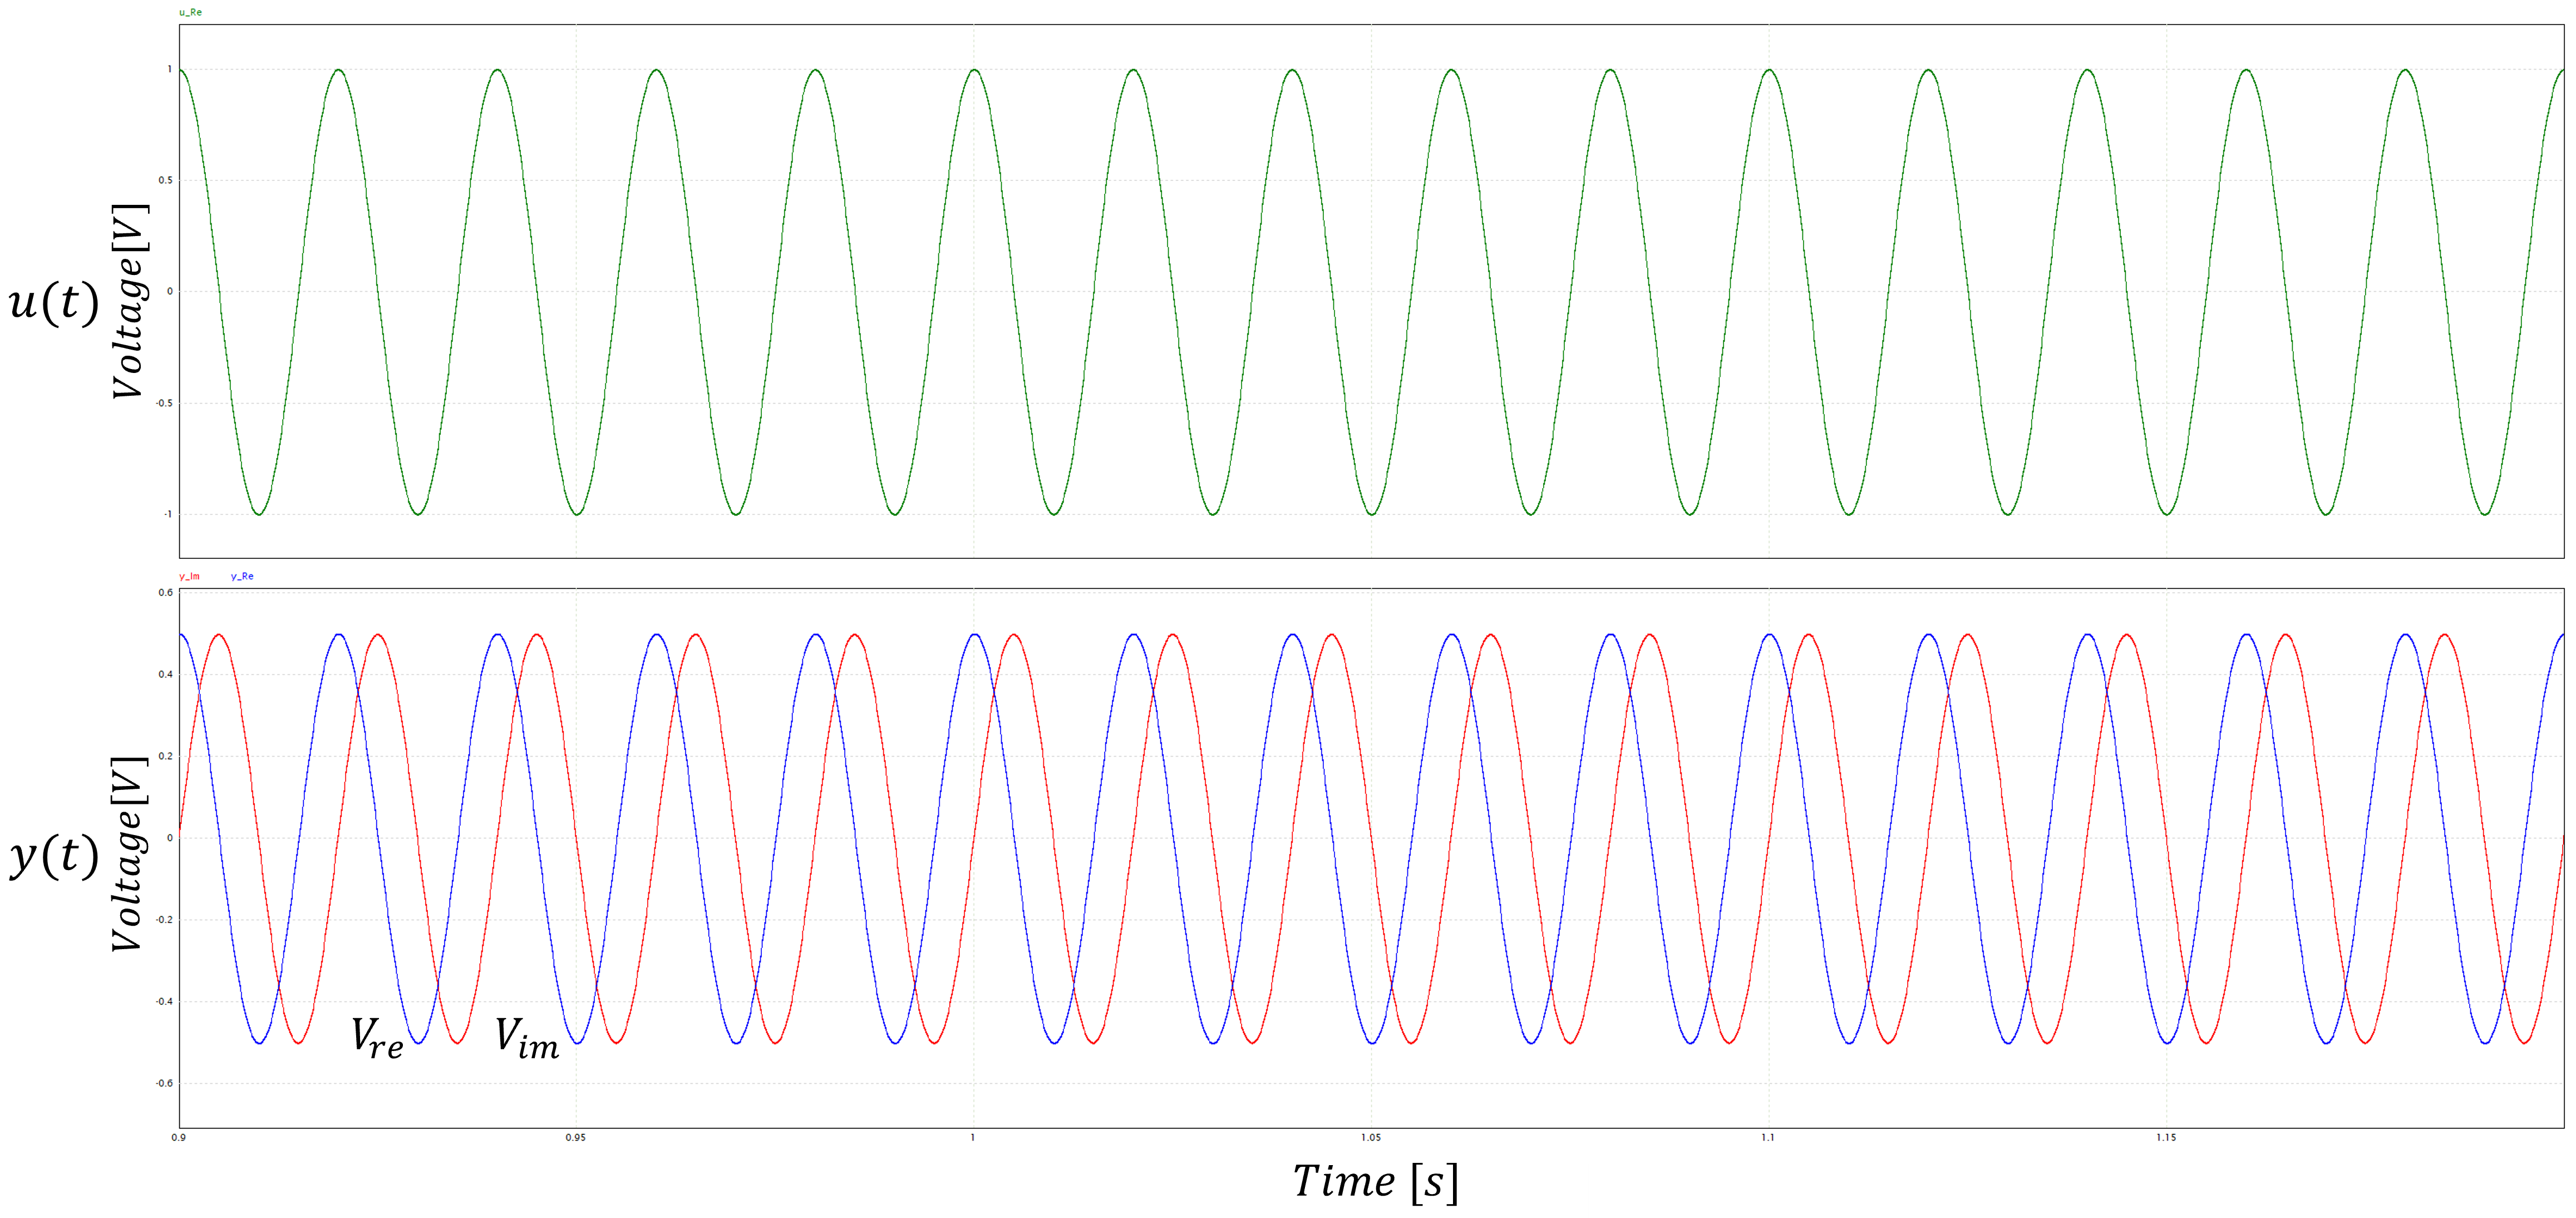
\includegraphics[width=0.5\textwidth]{figures/sim_no_h.png}
    \caption{Simulation results (without harmonic components)}
    \label{fig:without}
\end{figure}

\begin{figure}[htbp]
    \centering
     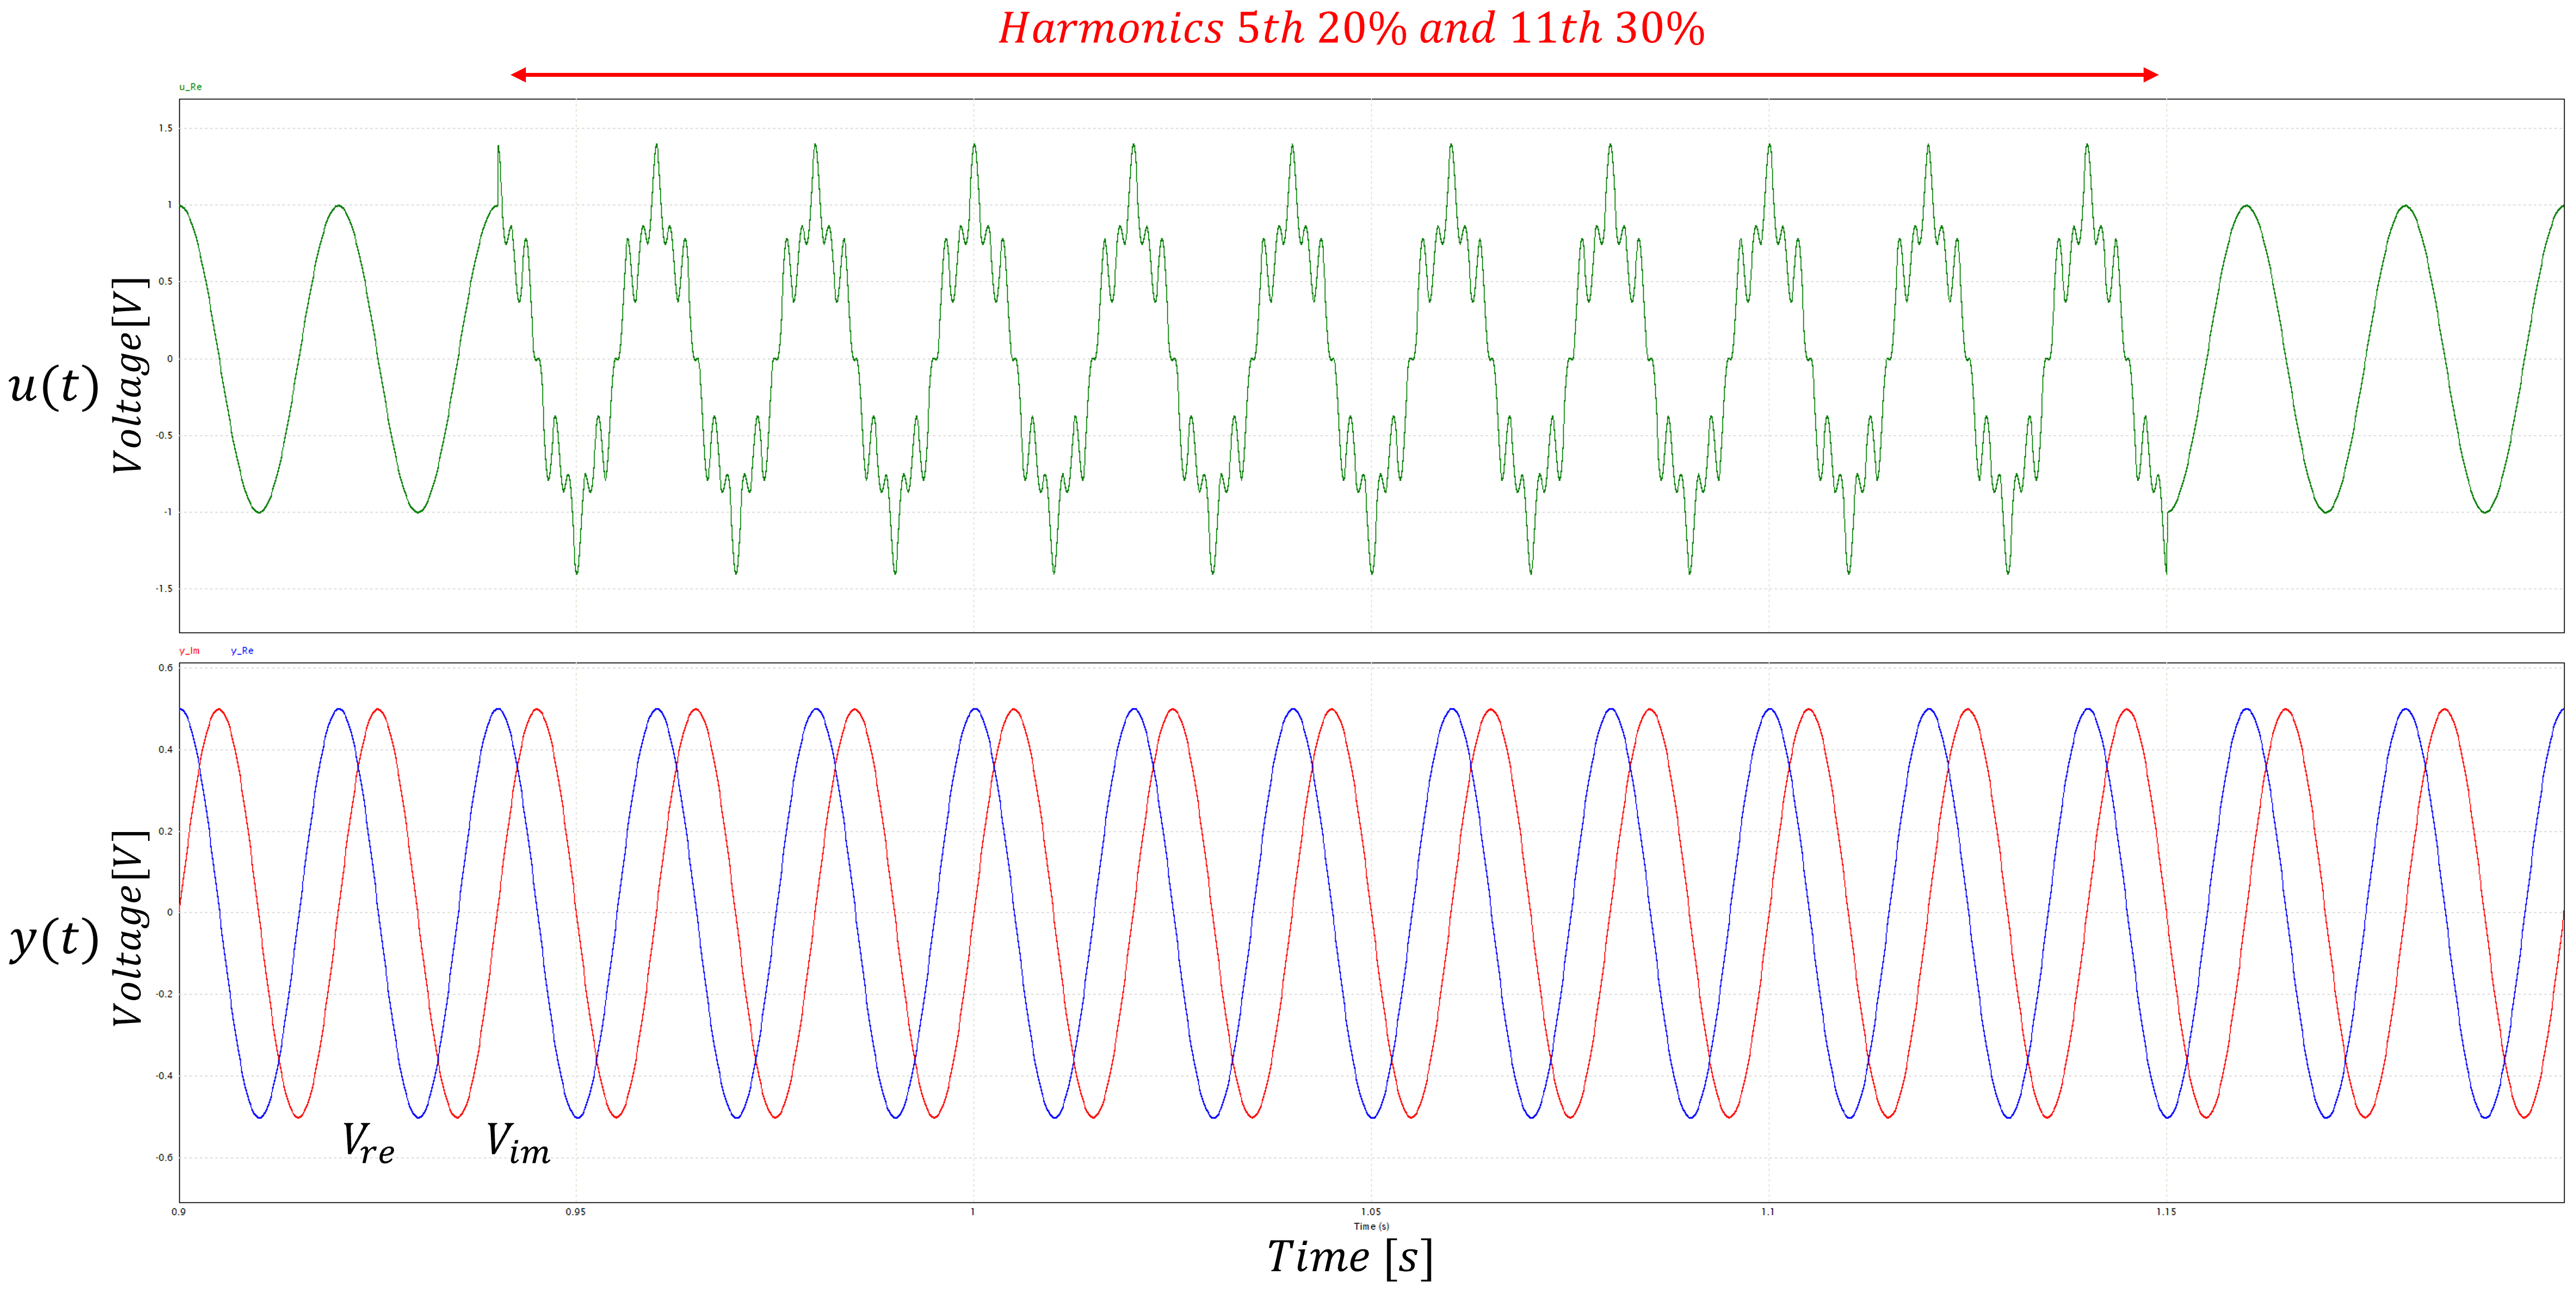
\includegraphics[width=0.5\textwidth]{figures/sim_with_h.png}
    \caption{Simulation results (with harmonic components)}
    \label{fig:with}
\end{figure}

\begin{figure}[htbp]
    \centering
     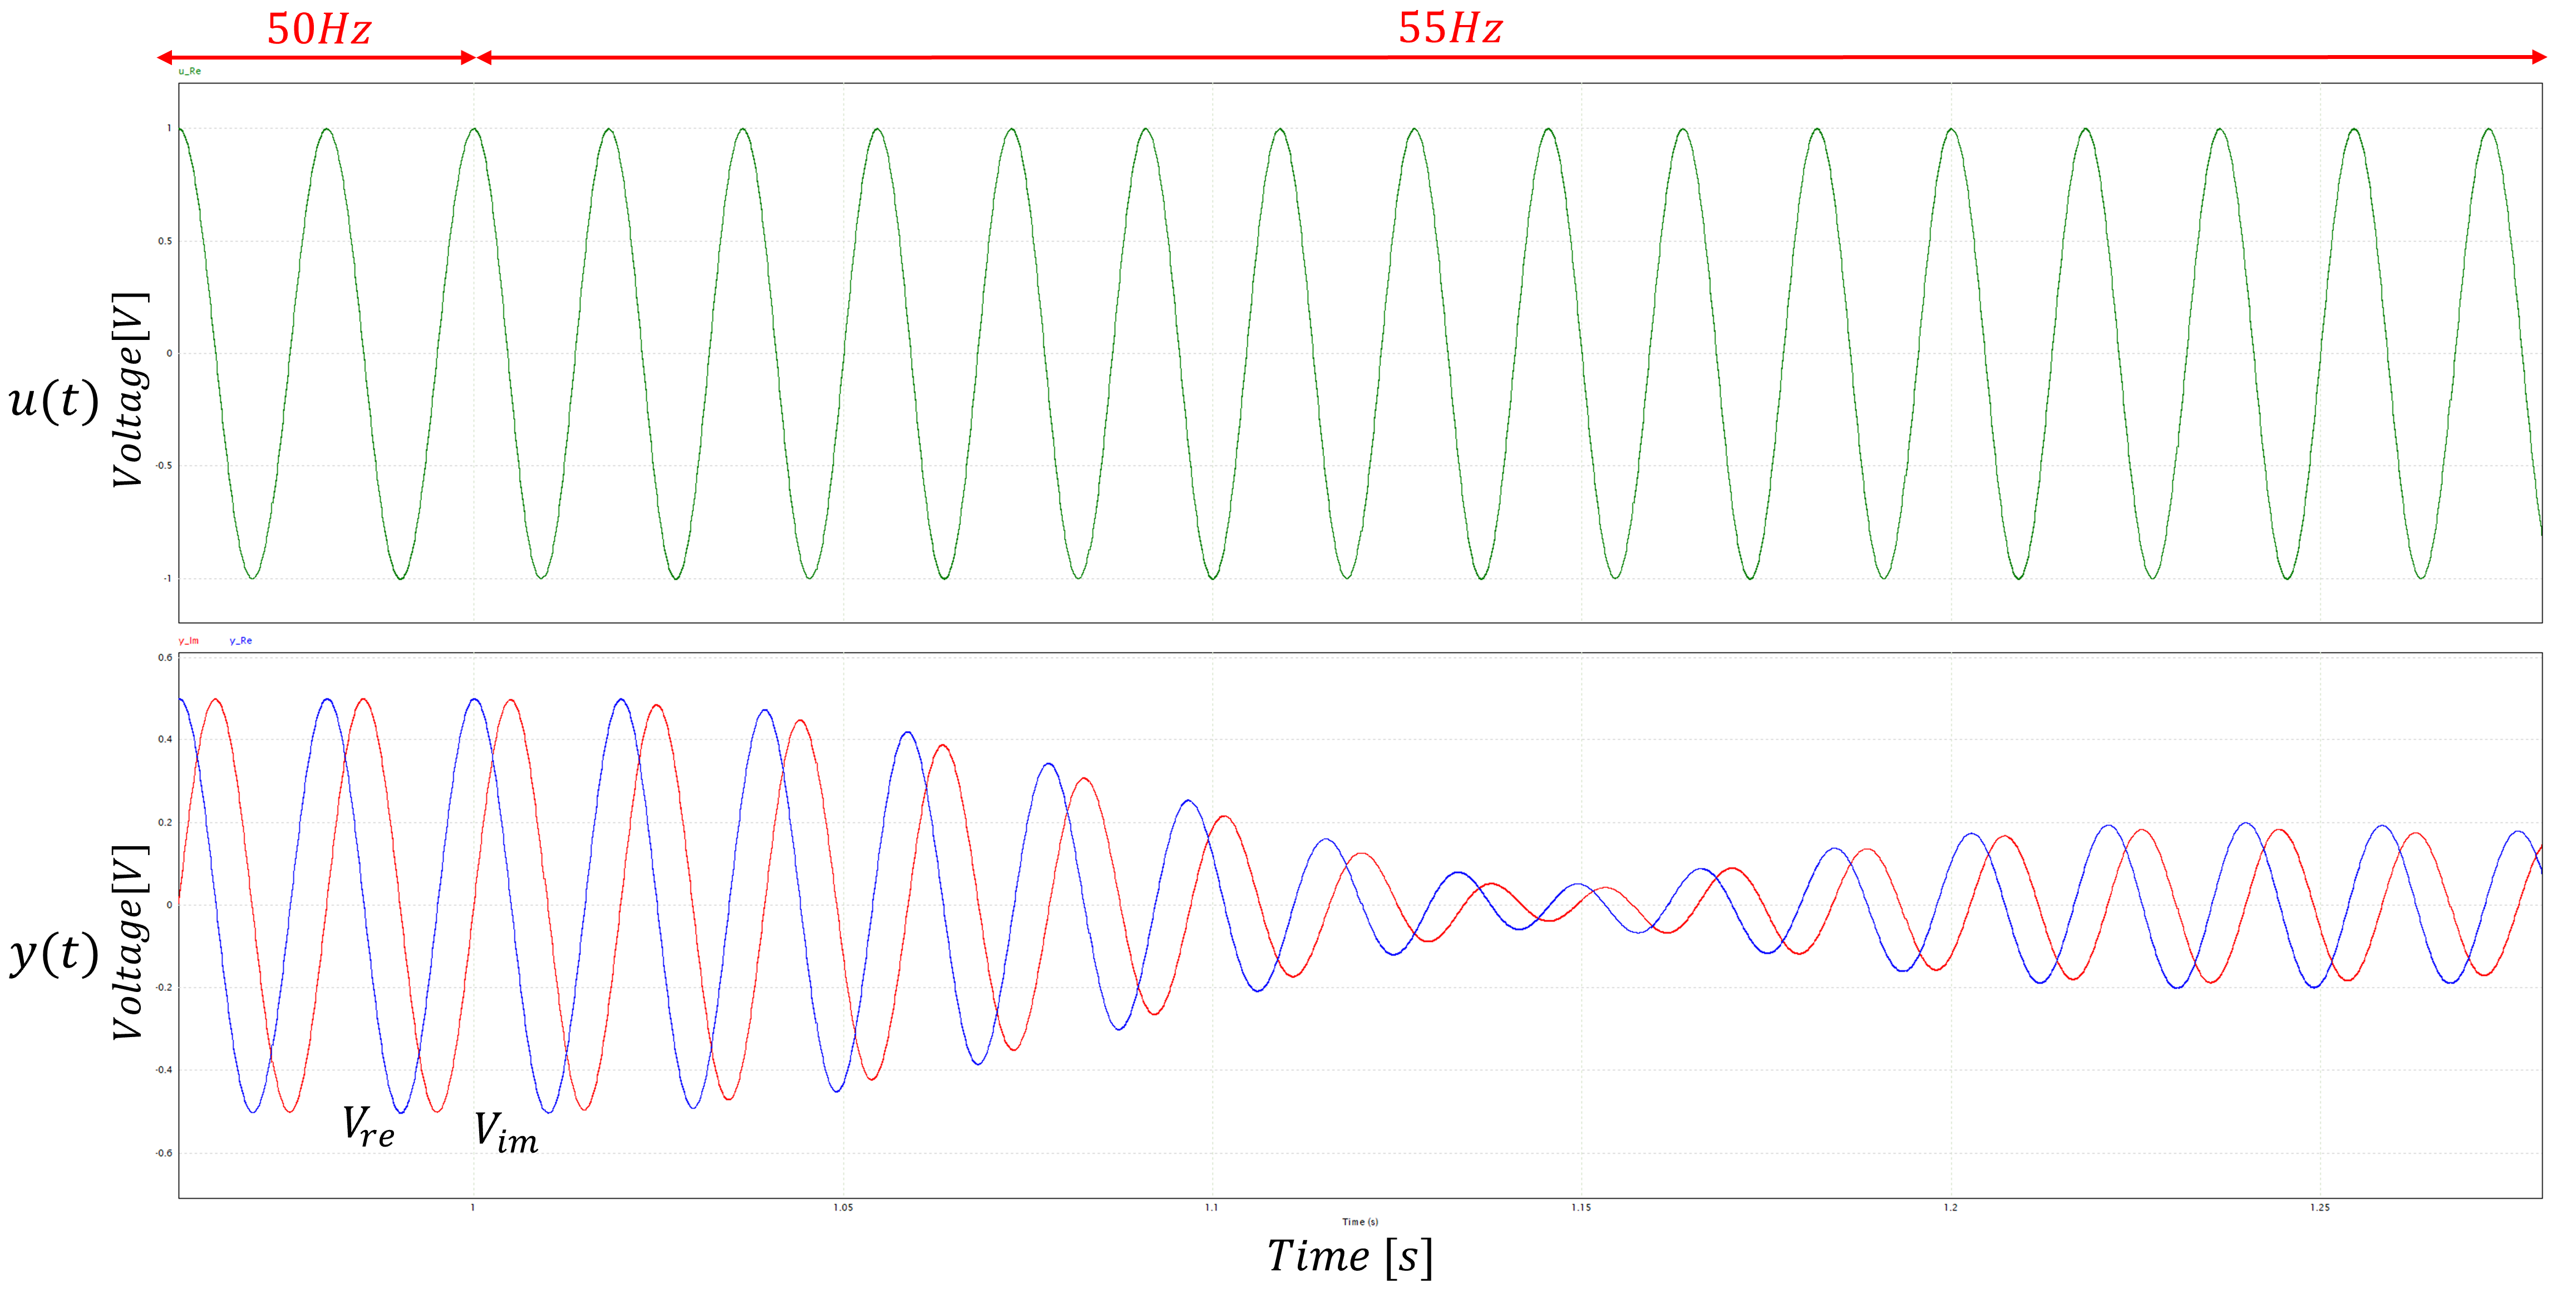
\includegraphics[width=0.5\textwidth]{figures/f_step.png}
    \caption{Simulation results (Frequency step from 50 Hz to 55 Hz)}
    \label{fig:f_step}
\end{figure}



